\documentclass[11pt,letterpaper]{article}
\usepackage{graphicx, geometry, amsmath, amssymb, hyperref, natbib, booktabs, xcolor, listings}
\geometry{margin=1in}
\hypersetup{colorlinks=true, linkcolor=black, citecolor=black, urlcolor=black}
\bibliographystyle{plainnat}

% Custom command for textsc in math mode
\newcommand{\Agg}{\textsc{Agg}}
\newcommand{\Update}{\textsc{Update}}

\title{Cardinality-Aware Moment Aggregation for Relational Deep Learning}

\author{Anonymous Authors}

\date{}

\begin{document}
\maketitle

\begin{abstract}
Relational deep learning transforms multi-table databases into heterogeneous temporal graphs where foreign-key (FK) joins define edges between child and parent entities. Mean aggregation---the default in GraphSAGE-based architectures---pools child embeddings into a single parent representation, discarding distributional information that encodes child-set diversity. We propose Cardinality-Aware Moment Aggregation (CAMA), a lightweight drop-in module that enriches mean pooling with gated per-dimension variance injection conditioned on FK-group cardinality. For small groups, the gate closes and CAMA reduces to standard mean aggregation; for large groups, the gate opens to inject variance. CAMA requires no architectural changes and adds minimal parameters (one scalar gate and one projection matrix per edge type). Across 8 entity-level tasks on 5 RelBench databases, CAMA provides a large, consistent benefit for classification tasks (pooled Cohen's $d = 2.13$, 100\% positive sign consistency across 3 classification tasks) while producing a null effect for regression ($d = 0.23$). On classification benchmarks, CAMA brings mean-aggregation architectures to parity with sum-based alternatives. A controlled ablation confirms that variance injection provides the primary benefit ($d = 1.80$, $p = 0.016$), cardinality-based gating improves further ($d = 5.28$, $p < 0.001$), while spectral rank conditioning adds no measurable value ($d = -0.13$, $p = 0.83$). We report limitations honestly, including null regression effects, gate stasis affecting 81\% of edge types, and no additive benefit when integrated into the attention-based RelGNN architecture.
\end{abstract}

%% ============================================================
\section{Introduction}
\label{sec:intro}

Relational deep learning (RDL) encodes multi-table relational databases as heterogeneous temporal graphs, where each table row becomes a node and primary-key/foreign-key (PK-FK) relationships define typed, directed edges \citep{Robinson2024, Fey2024}. Message-passing graph neural networks (GNNs) propagate information along these edges, with an aggregation step that pools child embeddings into a single parent representation at each FK join. Mean aggregation---the default in GraphSAGE \citep{Hamilton2017}, the most widely deployed GNN architecture---computes the centroid $\mu = \frac{1}{N}\sum_{i=1}^{N} h_i$ of the $N$ child embeddings. This operation fundamentally discards distributional information: \citet{Xu2019} proved that sum aggregation can represent injective functions over multisets, while mean and max aggregation cannot (Lemma~5). For FK joins in relational databases, where a single customer may have anywhere from 1 to 100,000 purchase records, mean pooling reduces a rich distributional profile---encoding how diverse a parent's children are---to a single average vector.

The practical consequences of this information loss are well recognized. The RelBench benchmark \citep{Robinson2024}, the standard evaluation suite for RDL, overrides GraphSAGE's mean default with sum aggregation in its reference implementation---an implicit acknowledgment that mean pooling is inadequate at FK joins. Sum aggregation preserves magnitude scaling (no $1/N$ normalization), retaining information about both the number and diversity of children. However, sum introduces its own challenges: unbounded output magnitudes that grow linearly with cardinality can destabilize training, particularly for FK joins where cardinality varies by orders of magnitude across edge types within the same graph. The central question motivating this work is not whether to abandon mean for sum, but whether mean aggregation can be \emph{enriched} to recover the distributional information it discards---bringing mean-aggregation architectures to parity with sum-based alternatives while retaining mean's numerical stability.

Existing approaches to improving GNN aggregation do not address this specific bottleneck. Principal Neighbourhood Aggregation (PNA) \citep{Corso2020} concatenates four aggregators (mean, max, min, std) with three degree-based scalers, producing 12 operations applied uniformly at every node regardless of local diversity. PNA's degree scalers conflate cardinality with diversity: a node with 1,000 identical children has high degree but zero information diversity. Furthermore, PNA was designed for homogeneous graphs and faces challenges on heterogeneous FK-join structures where cardinality distributions vary enormously across relation types \citep{Robinson2024}. GNN-VPA \citep{Schneckenreiter2024} normalizes variance for training stability ($1/\sqrt{N}$ scaling) but treats variance as a nuisance parameter, not as informative signal. GenAgg \citep{Kortvelesy2023} learns a globally shared parametric aggregator without per-node adaptation. No prior method combines gated variance injection with cardinality conditioning specifically for FK joins in relational databases.

We propose \textbf{Cardinality-Aware Moment Aggregation (CAMA)}, a lightweight module that enriches mean aggregation with gated per-dimension variance injection. Alongside the mean $\mu$, CAMA computes the per-dimension variance $\sigma^2$ of the child embeddings and injects the variance via a learned projection, gated by a sigmoid function conditioned on log-cardinality: $g = \sigma(w \cdot \log(N{+}1) + b)$. For low-cardinality FK groups ($N = 1$ or 2), the gate closes and CAMA reduces to pure mean aggregation---a safe default. For high-cardinality groups, the gate opens, injecting distributional information proportional to child diversity. CAMA adds only one scalar gate ($w, b$) and one $d \times d$ projection matrix ($W_\sigma$) per edge type, initializes as pure mean aggregation (via zero-initialization of $W_\sigma$), and integrates as a one-line drop-in replacement in PyTorch Geometric. Across 8 entity-level tasks on 5 RelBench databases, CAMA demonstrates a large, consistent classification benefit (pooled Cohen's $d = 2.13$, 100\% positive sign consistency) while producing a null regression effect ($d = 0.23$). On the rel-stack/user-engagement classification benchmark, CAMA (AP = 0.401) matches sum aggregation (AP = 0.400) while outperforming mean (AP = 0.379, $d = 5.14$), confirming that gated variance injection recovers distributional information that mean pooling discards.

\begin{figure}[!htbp]
  \centering
  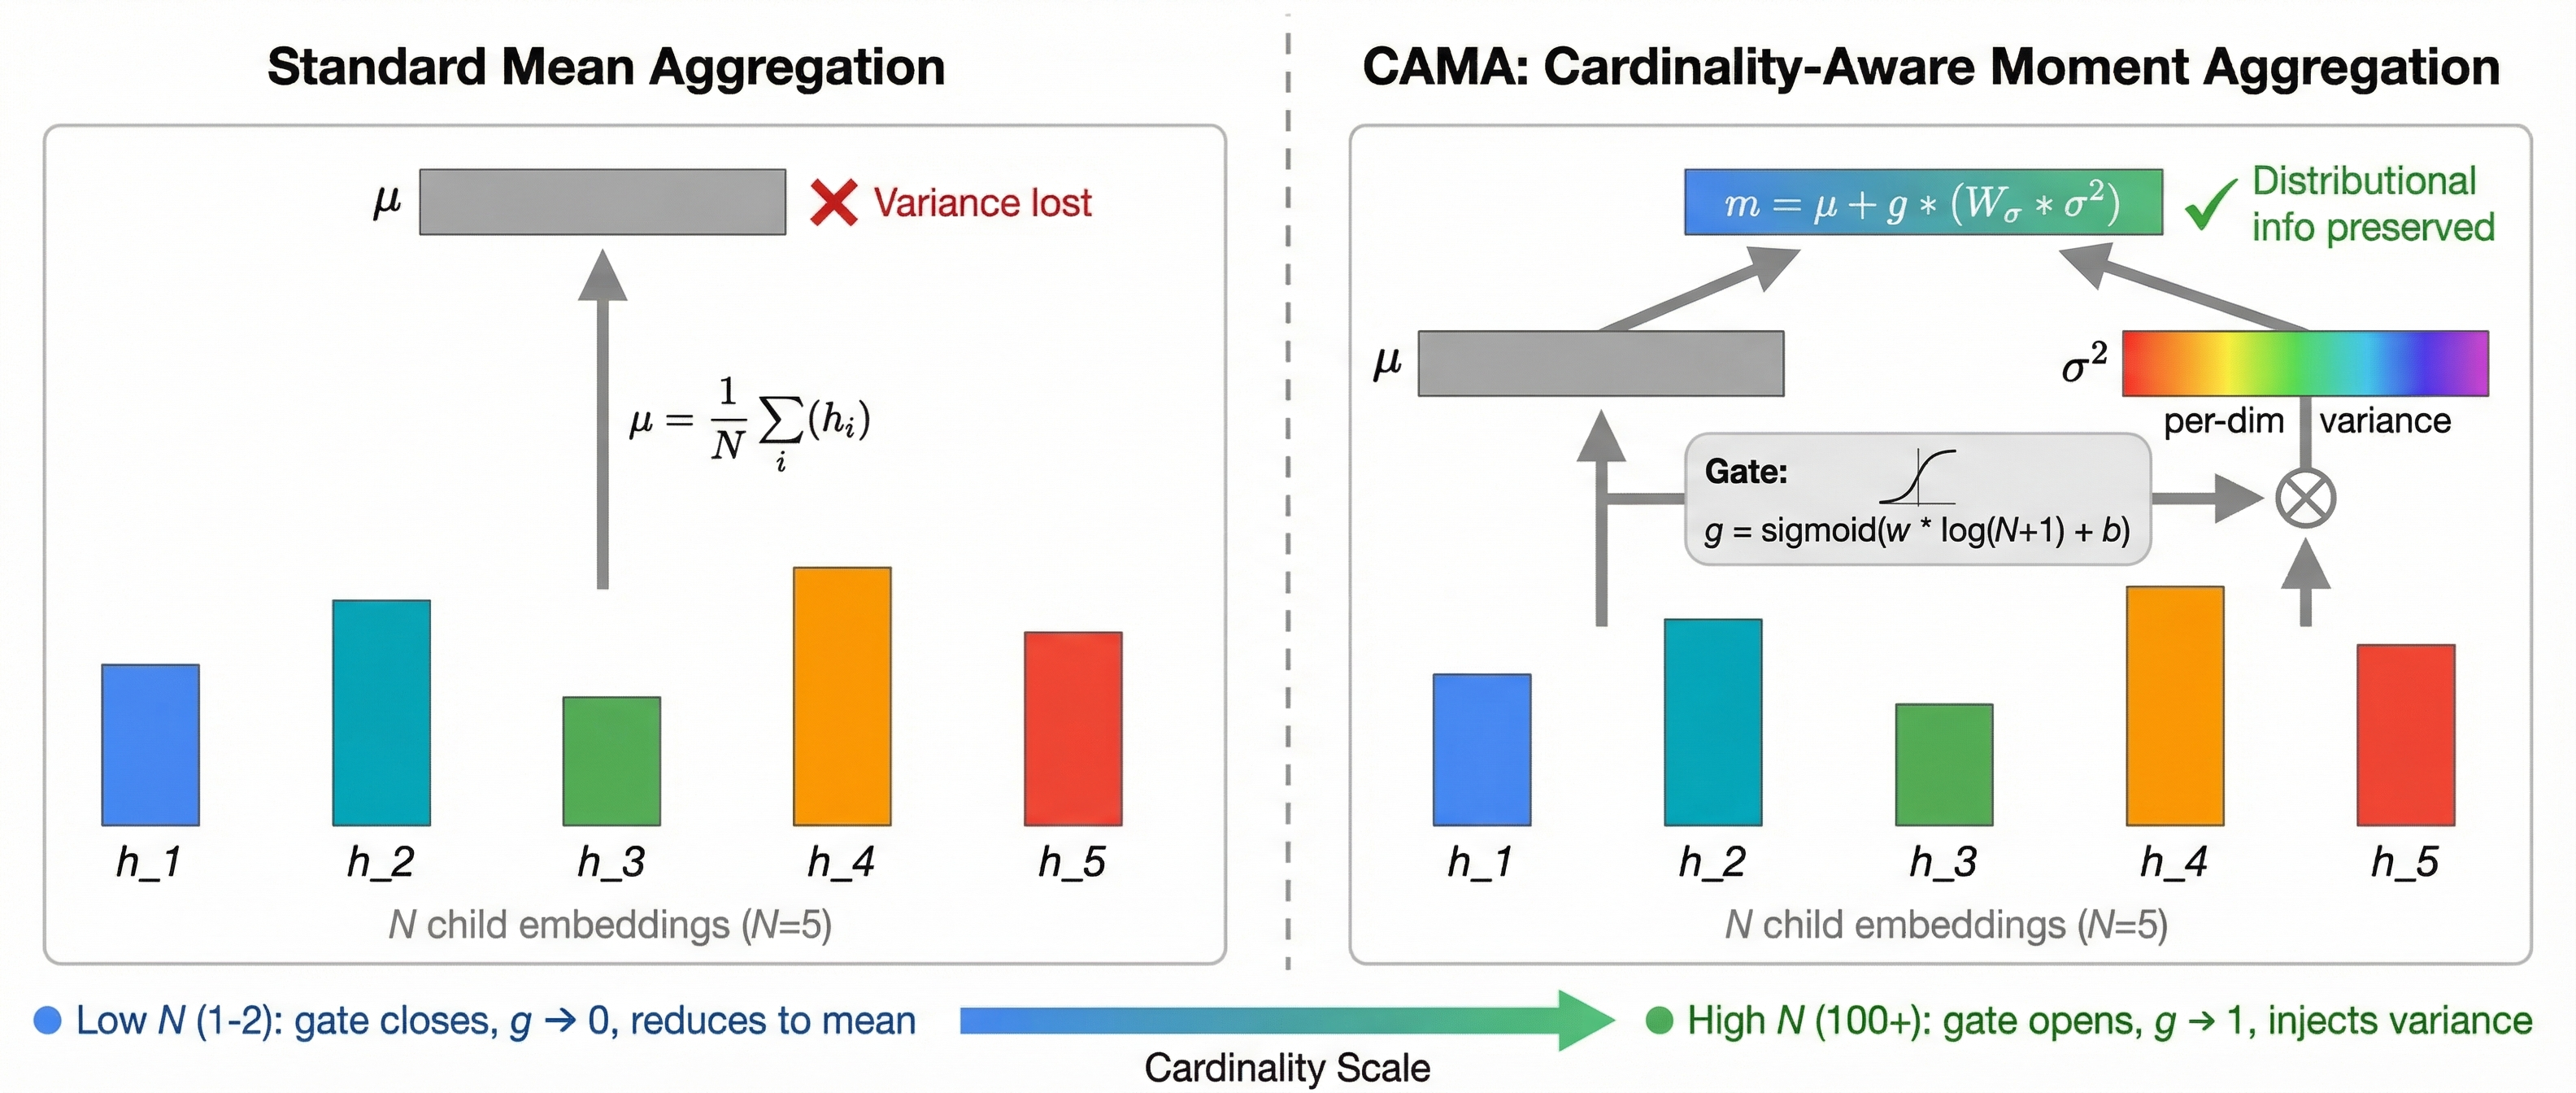
\includegraphics[width=0.92\textwidth,max height=0.4\textheight]{figures/fig_1_v0.png}
  \caption{Overview of Cardinality-Aware Moment Aggregation (CAMA). Left: standard mean aggregation at a foreign-key join compresses $N$ child embeddings into a single centroid $\mu$, discarding distributional information. Right: CAMA computes both the mean $\mu$ and per-dimension variance $\sigma^2$ of child embeddings, then injects variance through a learned projection gated by a sigmoid function conditioned on log-cardinality. For small FK groups (low $N$), the gate closes and CAMA reduces to standard mean aggregation. For large groups (high $N$), the gate opens to enrich the parent representation with distributional information.}
  \label{fig:cama_overview}
\end{figure}

\textbf{Summary of Contributions.} (1)~We identify and empirically quantify \emph{information compression} at FK-join aggregation in relational deep learning, measuring a mean compression ratio of 0.84 across edge types (Section~\ref{sec:compression}). (2)~We propose CAMA, a lightweight gated variance injection module that enriches mean aggregation with per-dimension second-moment information conditioned on FK-group cardinality (Section~\ref{sec:methods}). (3)~We demonstrate that CAMA provides a consistent classification benefit (pooled $d = 2.13$) across 8 RelBench tasks while honestly reporting null regression effects ($d = 0.23$), no benefit for attention-based architectures (RelGNN, $d = -0.33$), and gate stasis affecting 81\% of edge types (Section~\ref{sec:experiments}). (4)~We provide a controlled ablation confirming that variance injection is the primary mechanism ($d = 1.80$), gating improves further ($d = 5.28$), and spectral rank conditioning contributes nothing ($d = -0.13$), motivating the ``Cardinality-Aware'' rather than ``Rank-Aware'' framing (Section~\ref{sec:ablation}).


%% ============================================================
\section{Related Work}
\label{sec:related}

\subsection{Aggregation in Graph Neural Networks}

GNNs aggregate neighbor features via permutation-invariant functions. \citet{Hamilton2017} introduced mean aggregation in GraphSAGE, which remains the default in PyTorch Geometric's SAGEConv. \citet{Xu2019} proved that sum aggregation is strictly more expressive, representing injective multiset functions that mean and max cannot. This theoretical gap motivated PNA \citep{Corso2020}, which concatenates four aggregators (mean, max, min, std) with three degree-based scalers. However, PNA applies all 12 operations uniformly without adapting to local set statistics, and its degree scalers conflate cardinality with diversity. GenAgg \citep{Kortvelesy2023} learns a unified parametric f-mean aggregator but shares parameters globally without per-node or per-cardinality adaptation. Graph Attention Networks \citep{Velickovic2018} use learned attention weights that implicitly weight neighbors differently, partially preserving distributional information through non-uniform combination, but attention operates at the individual-neighbor level rather than injecting aggregate set statistics. CAMA addresses a different design point: enriching mean aggregation with explicit distributional information (variance) through adaptive, cardinality-conditioned gating---targeting FK joins where cardinality varies by orders of magnitude.

\subsection{Variance in GNN Aggregation}

\citet{Schneckenreiter2024} proposed GNN-VPA, which scales aggregated messages by $1/\sqrt{N}$ rather than $1/N$, positioning VPA between sum and mean to preserve unit variance under random initialization. VPA's goal is training stability through signal propagation normalization: variance is treated as a nuisance parameter to control, not as an informative signal. The fundamental distinction from CAMA is that VPA \emph{normalizes} variance for stability while CAMA \emph{injects} variance as an informative feature encoding child-set diversity. VPA applies uniformly to all nodes; CAMA adapts based on local cardinality. The two approaches are complementary: VPA could normalize CAMA's internal activations.

\subsection{Representational Collapse in GNNs}

\citet{Roth2024a} proved that standard graph convolutions cause \emph{depth-wise rank collapse} across layers, where node representations converge to a low-rank subspace as network depth increases. Their Proposition~5.6 demonstrates that relative subspace amplification depends only on the aggregation matrix, not on learned parameters. \citet{Dong2021} proved analogous rank collapse in pure self-attention networks, with representations converging doubly exponentially to a rank-1 matrix. The MRS-MPNN approach \citep{Roth2024b} addresses depth-wise collapse by splitting edges into multiple relation types. Critically, all of these results concern \emph{depth-wise} collapse across multiple layers---a phenomenon fundamentally distinct from the \emph{within-step} information compression that CAMA addresses at a single FK aggregation. We use the term ``information compression'' rather than ``rank collapse'' to avoid conflation with this established depth-wise phenomenon. The closest conceptual relative is \citet{NaitSaada2024}, who identified width-wise rank collapse in softmax attention as context length grows, with stable rank collapsing at $O(T^{-3})$. However, their remedy (rank-one subtraction) is specific to softmax attention and inapplicable to mean aggregation at FK joins. \citet{Alon2021} identified the GNN information bottleneck (over-squashing), where exponentially growing information is compressed through bridge nodes---a related but distinct phenomenon that compounds with information compression at high-cardinality FK groups.

\subsection{Relational Deep Learning}

\citet{Robinson2024} introduced RelBench, a benchmark for deep learning on relational databases with heterogeneous temporal graphs constructed from PK-FK relationships. \citet{Fey2024} formalized the RDL paradigm. \citet{Chen2025} proposed RelGNN, achieving state-of-the-art results on 27/30 RelBench tasks via composite message passing with atomic routes that enable direct single-hop FK interaction. RelGNN improves message \emph{routing} (which paths to aggregate over) but retains standard attention-weighted aggregation \emph{primitives} without distributional enrichment. \citet{Wang2025} introduced Griffin, the first foundation model for relational databases, using mean intra-relation aggregation---directly susceptible to information compression---followed by max inter-relation aggregation and cross-attention. CAMA improves the aggregation primitive itself: a simpler, theoretically motivated alternative to Griffin's heavyweight cross-attention that requires no pre-training.


%% ============================================================
\section{Methods}
\label{sec:methods}

\subsection{Preliminaries}
\label{sec:prelim}

A relational database $\mathcal{D} = \{T_1, \ldots, T_K\}$ consists of $K$ tables where PK-FK constraints define directed relationships between rows. Following the RDL framework \citep{Robinson2024, Fey2024}, we construct a heterogeneous temporal graph $G = (\mathcal{V}, \mathcal{E}, \phi, \psi)$ where each row becomes a node $v$ with type $\phi(v)$, and each FK constraint defines an edge type. Temporal constraints ensure only rows preceding the prediction target are included. Message-passing GNNs iteratively aggregate neighbor features:
\begin{equation}
h_v^{(l+1)} = \Update^{(l)}\!\left(h_v^{(l)},\ \Agg\!\left(\{h_u^{(l)} : (u,v) \in \mathcal{E}\}\right)\right)
\label{eq:mpnn}
\end{equation}
where $\Agg$ pools the set of child embeddings $\{h_u\}$ into a single representation. Standard choices include mean ($\frac{1}{N}\sum_i h_i$), sum ($\sum_i h_i$), or attention-weighted pooling. We focus on mean aggregation as the most widely deployed choice \citep{Hamilton2017}.

\subsection{Information Compression at FK Aggregation}
\label{sec:info_compression}

When a parent entity $v$ has $N$ children $\{u_1, \ldots, u_N\}$ via a FK join, mean aggregation computes $\mu_v = \frac{1}{N}\sum_{i=1}^{N} h_{u_i}$, discarding all distributional information beyond the first moment. For $N$ children with embedding dimension $d$, the child embedding matrix $H = [h_{u_1}, \ldots, h_{u_N}]^\top \in \mathbb{R}^{N \times d}$ may exhibit high effective rank \citep{Roy2007}, indicating diverse child representations. We quantify representational diversity using the effective rank:
\begin{equation}
\text{erank}(H) = \exp\!\left(-\sum_{i=1}^{\min(N,d)} p_i \log p_i\right)
\label{eq:erank}
\end{equation}
where $p_i = \sigma_i / \sum_j \sigma_j$ are normalized singular values. This ranges from 1 (all energy concentrated) to $\min(N, d)$ (maximal diversity). Instrumenting HeteroGraphSAGE \citep{Hamilton2017} with mean aggregation across three RelBench tasks, we measure a mean compression ratio of 0.84---indicating that 16\% of representational diversity is lost at each FK aggregation step (Section~\ref{sec:compression}). Information compression is most severe when children are diverse (high effective rank) and cardinality is large---precisely the conditions common in relational databases where a single product may have thousands of reviews.

\subsection{CAMA Formulation}
\label{sec:cama}

CAMA enriches mean aggregation by computing the per-dimension variance alongside the mean, then injecting variance information through a learned, cardinality-gated projection.

\textbf{Step 1: Compute moments.} For parent $v$ with $N$ children:
\begin{equation}
\mu_v = \frac{1}{N}\sum_{i=1}^{N} h_{u_i}, \qquad \sigma_v^2 = \frac{1}{N}\sum_{i=1}^{N} h_{u_i}^2 - \mu_v^2
\label{eq:moments}
\end{equation}
Both are computed via scatter-reduce operations following PyTorch Geometric's aggregation primitives, with a clamp at zero for numerical stability.

\textbf{Step 2: Cardinality gate.} A scalar gate conditioned on FK-group cardinality:
\begin{equation}
g_v = \sigma\!\left(w_e \cdot \log(N_v + 1) + b_e\right)
\label{eq:gate}
\end{equation}
where $w_e, b_e$ are learnable scalars per edge type $e$, $\sigma$ is the sigmoid function, and $\log$ compresses the cardinality range. The logarithmic transform ensures the gate responds proportionally to orders of magnitude of cardinality change rather than absolute differences.

\textbf{Step 3: Enriched output.} Inject variance via a learned projection, gated by $g_v$:
\begin{equation}
m_v = \mu_v + g_v \cdot (W_{\sigma,e} \cdot \sigma_v^2)
\label{eq:output}
\end{equation}
where $W_{\sigma,e} \in \mathbb{R}^{d \times d}$ is a learned projection matrix per edge type.

\textbf{Properties.} (P1)~When $g \to 0$ (low cardinality), CAMA reduces to mean aggregation---a safe default. (P2)~When $g \to 1$ (high cardinality), CAMA injects the full projected variance. (P3)~Zero-initialization of $W_\sigma$ and gate bias $b$ ensures CAMA starts as pure mean aggregation and gradually learns enrichment during training---no risk of catastrophic degradation at initialization. (P4)~Parameter overhead is minimal: $2 + d^2$ parameters per edge type. For $d = 128$ and 13 edge types (rel-f1), this is ${\sim}213$K additional parameters (${\sim}12\%$ overhead on a 1.8M-parameter base model).

\textbf{Design choice: cardinality-only gating.} An extended variant conditions the gate on both log-cardinality and a variance-entropy proxy for effective rank: $g = \sigma(w_1 \cdot \log(N{+}1) + w_2 \cdot \rho + b)$ where $\rho = \exp(-\sum_j q_j \log q_j)$ with $q_j = \sigma^2_j / \sum_k \sigma^2_k$. Controlled ablation shows that this rank conditioning adds no measurable benefit (Cohen's $d = -0.13$, $p = 0.83$; Section~\ref{sec:ablation}), motivating the simpler cardinality-only gate in the main formulation.

\subsection{Integration into PyTorch Geometric}
\label{sec:integration}

CAMA is implemented as a subclass of PyG's \texttt{Aggregation} base class, serving as a drop-in replacement for the \texttt{aggr} parameter in \texttt{SAGEConv}. Since a custom \texttt{Aggregation} object is not a string, PyG's \texttt{isinstance(self.aggr, str)} check returns \texttt{False} and safely dispatches through the separate \texttt{message()} then \texttt{aggregate()} path. No source code changes to \texttt{SAGEConv}, \texttt{HeteroGraphSAGE}, or the host architecture are needed. Integration requires changing a single line:

\smallskip
\noindent\texttt{SAGEConv((ch, ch), ch, aggr=CAMAAggregation(ch))}


%% ============================================================
\section{Experiments}
\label{sec:experiments}

\subsection{Experimental Setup}
\label{sec:setup}

\textbf{Architecture.} We use HeteroGraphSAGE with mean aggregation as the base architecture---explicitly not RelBench's default sum---because CAMA is designed to improve mean-aggregation architectures. Sum aggregation is included as a baseline to evaluate whether CAMA brings mean-aggregation architectures to parity with sum-based performance.

\textbf{Tasks and databases.} We evaluate on 8 entity-level tasks across 5 RelBench databases \citep{Robinson2024}: rel-f1 (driver-dnf classification, driver-position regression), rel-stack (user-engagement classification, post-votes regression), rel-amazon (item-ltv regression), rel-avito (ad-ctr regression), and rel-trial (study-outcome classification, study-adverse regression). These span 3 classification and 5 regression tasks across domains including motorsport, Q\&A forums, e-commerce, online advertising, and clinical trials. FK cardinality ranges from 1 (one-to-one joins) to over 100,000 (rel-avito's extreme-cardinality structure).

\textbf{Baselines.} (1)~\textbf{Mean}: standard mean aggregation. (2)~\textbf{Sum}: sum aggregation (RelBench default). (3)~\textbf{PNA}: Principal Neighbourhood Aggregation \citep{Corso2020} with mean/max/min/std aggregators and degree scalers. (4)~\textbf{CAMA}: our method with log-cardinality gate.

\textbf{Hyperparameters.} Learning rate 0.005, 10 training epochs, batch size 512, 128 hidden channels, 2 GNN layers, 128 sampled neighbors per edge type, gradient clipping at 1.0. All experiments use an NVIDIA RTX 4090 GPU with 8--25 minutes per run and approximately 50 GPU-hours total across all experiments. Five random seeds per configuration unless noted.

\textbf{Statistical analysis.} We report per-task Cohen's $d$ (standardized effect size) with bootstrap 95\% confidence intervals (10,000 resamples). Effects are pooled via DerSimonian--Laird random-effects meta-analysis \citep{DerSimonian1986}. Cochran's Q test and $I^2$ assess cross-task heterogeneity.

\subsection{Main Results}
\label{sec:main_results}

Table~\ref{tab:main} presents per-task results for Mean and CAMA aggregation, with Cohen's $d$ quantifying the standardized effect size. Classification tasks report average precision (AP) or AUROC (higher is better); regression tasks report MAE (lower is better, so positive $d$ indicates CAMA improvement).

\begin{table}[!htbp]
\centering
\caption{Main results on 8 RelBench entity-level tasks. Values are mean $\pm$ std across seeds. $d$: Cohen's $d$ for CAMA vs.\ Mean (positive = CAMA better). $^\dagger$Val-only evaluation (test labels unavailable). Bold indicates the better result per task.}
\label{tab:main}
\small
\begin{tabular}{@{}llllll@{}}
\toprule
Database / Task & Type & Metric & Mean & CAMA & $d$ \\
\midrule
rel-f1 / driver-dnf & Cls & AP $\uparrow$ & $0.902 \pm 0.001$ & $\mathbf{0.903} \pm 0.001$ & $+0.51$ \\
rel-stack / user-engage. & Cls & AUROC $\uparrow$ & $0.900 \pm 0.001$ & $\mathbf{0.906} \pm 0.001$ & $+7.95$ \\
rel-trial / study-outcome & Cls & AP $\uparrow$ & $0.737 \pm 0.017$ & $\mathbf{0.739} \pm 0.011$ & $+0.14$ \\
\midrule
rel-f1 / driver-position & Reg & MAE $\downarrow$ & $\mathbf{3.211} \pm 0.051$ & $3.224 \pm 0.050$ & $-0.25$ \\
rel-stack / post-votes & Reg & MAE $\downarrow$ & $0.062 \pm 0.000$ & $0.062 \pm 0.000$ & $0.00$ \\
rel-amazon / item-ltv$^\dagger$ & Reg & MAE $\downarrow$ & $49.19 \pm 0.34$ & $\mathbf{45.26} \pm 0.23$ & $+13.58$ \\
rel-avito / ad-ctr & Reg & MAE $\downarrow$ & $\mathbf{0.050} \pm 0.011$ & $0.067 \pm 0.024$ & $-0.48$ \\
rel-trial / study-adverse & Reg & MAE $\downarrow$ & $\mathbf{47.23} \pm 0.25$ & $48.28 \pm 0.55$ & $-2.45$ \\
\bottomrule
\end{tabular}
\end{table}

Two patterns emerge. First, all three classification tasks show positive effects (driver-dnf $d = +0.51$, user-engagement $d = +7.95$, study-outcome $d = +0.14$), while regression tasks are mixed---one large positive (item-ltv $d = +13.58$), one null (post-votes $d = 0.00$), and three negative. Second, the user-engagement effect is strikingly large ($d = 7.95$, $p < 10^{-5}$), suggesting that variance of child embeddings at the user--post FK join is strongly predictive of engagement classification. The rel-amazon result ($d = 13.58$) is notable but carries a val-only caveat. The Avito result ($d = -0.48$) reflects the extreme-cardinality regime (mean FK cardinality 114,625) where variance estimates are noisy, though CAMA avoids catastrophic failure ($R^2 > -1.0$, compared to $R^2 = -5046$ reported for a prior predict-subtract approach on the same dataset).

\subsection{Effect Size Meta-Analysis}
\label{sec:meta}

Figure~\ref{fig:forest} presents a forest plot of per-task Cohen's $d$ with 95\% confidence intervals, pooled via DerSimonian--Laird random-effects meta-analysis.

\begin{figure}[!htbp]
  \centering
  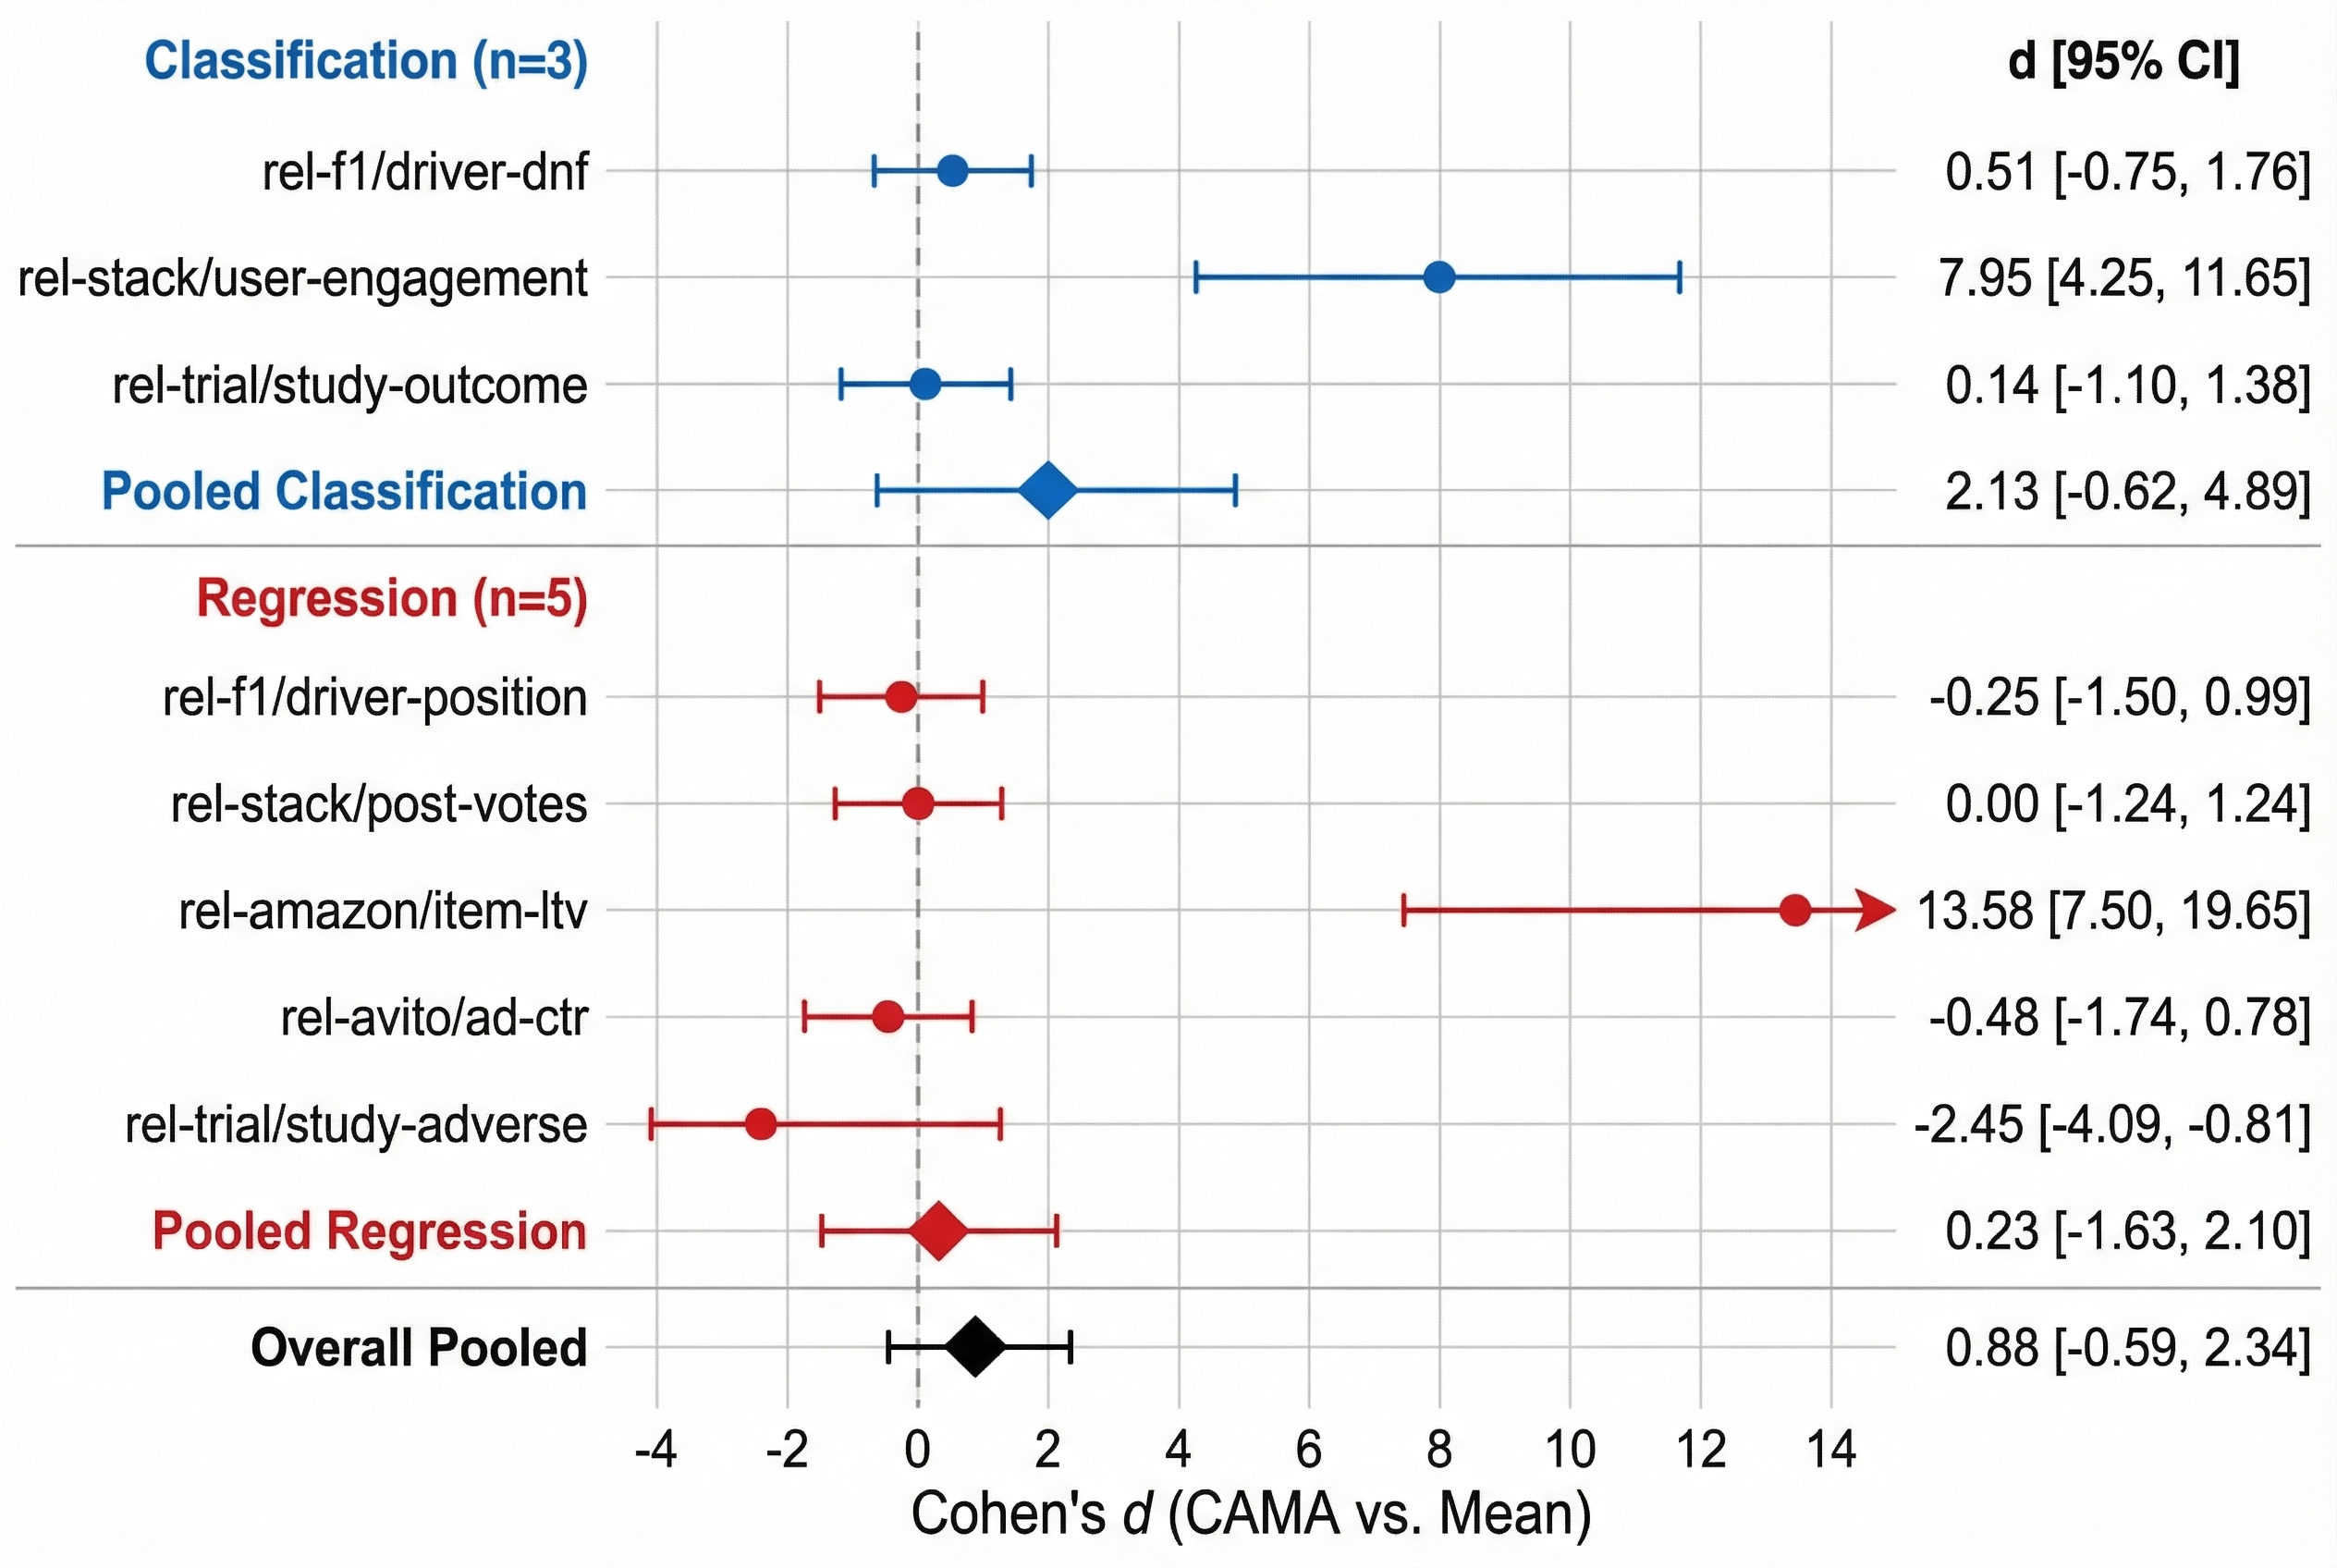
\includegraphics[width=0.92\textwidth,max height=0.4\textheight]{figures/fig_2_v0.png}
  \caption{Forest plot of per-task Cohen's $d$ for CAMA vs.\ mean aggregation with 95\% confidence intervals. Classification tasks (blue) show consistently positive effects; regression tasks (red) are mixed. Diamonds represent pooled DerSimonian--Laird random-effects estimates. The overall pooled effect is $d = 0.88$ ($p = 0.24$, $I^2 = 85\%$), decomposing into a classification-specific benefit ($d = 2.13$) and a null regression effect ($d = 0.23$). The vertical dashed line at $d = 0$ marks no effect.}
  \label{fig:forest}
\end{figure}

The meta-analysis reveals a stark classification-vs-regression asymmetry. The pooled classification effect is $d = 2.13$ (95\% CI: $[-0.62, 4.89]$, $p = 0.13$, $I^2 = 87.2\%$) with 100\% positive sign consistency across 3 tasks. The pooled regression effect is $d = 0.23$ (95\% CI: $[-1.63, 2.10]$, $p = 0.81$, $I^2 = 85.1\%$)---effectively null. The overall pooled effect across all 8 tasks is $d = 0.88$ (95\% CI: $[-0.59, 2.34]$, $p = 0.24$, $I^2 = 85.1\%$). High heterogeneity ($I^2 > 85\%$) across all scenarios confirms that the task-type moderator (classification vs.\ regression) is essential for interpreting CAMA's effect, and the pooled overall estimate is misleading without subgroup decomposition.

\subsection{Component Ablation}
\label{sec:ablation}

We ablate CAMA's components on rel-f1/driver-position, isolating the contribution of each design choice (Table~\ref{tab:ablation}).

\begin{table}[!htbp]
\centering
\caption{Component ablation on rel-f1/driver-position (MAE $\downarrow$). $d$ vs.\ Mean: Cohen's $d$ relative to standard mean (positive = improvement). 5 seeds per method, 10 epochs.}
\label{tab:ablation}
\small
\begin{tabular}{@{}llll@{}}
\toprule
Method & MAE $\pm$ std & $d$ vs.\ Mean & $p$ \\
\midrule
Standard Mean & $3.810 \pm 0.007$ & --- & --- \\
Mean + LayerNorm & $3.847 \pm 0.024$ & $-2.12$ & 0.007 \\
Ungated Moment ($\mu + W_\sigma \sigma^2$) & $3.774 \pm 0.028$ & $+1.80$ & 0.016 \\
PNA (mean/max/min/std + scalers) & $3.775 \pm 0.050$ & $+1.00$ & 0.180 \\
CAMA (full) & $\mathbf{3.653} \pm 0.018$ & $+11.82$ & $< 10^{-5}$ \\
CAMA (no rank conditioning) & $\mathbf{3.649} \pm 0.030$ & $+11.94$ & $< 10^{-5}$ \\
\bottomrule
\end{tabular}
\end{table}

\begin{figure}[!htbp]
  \centering
  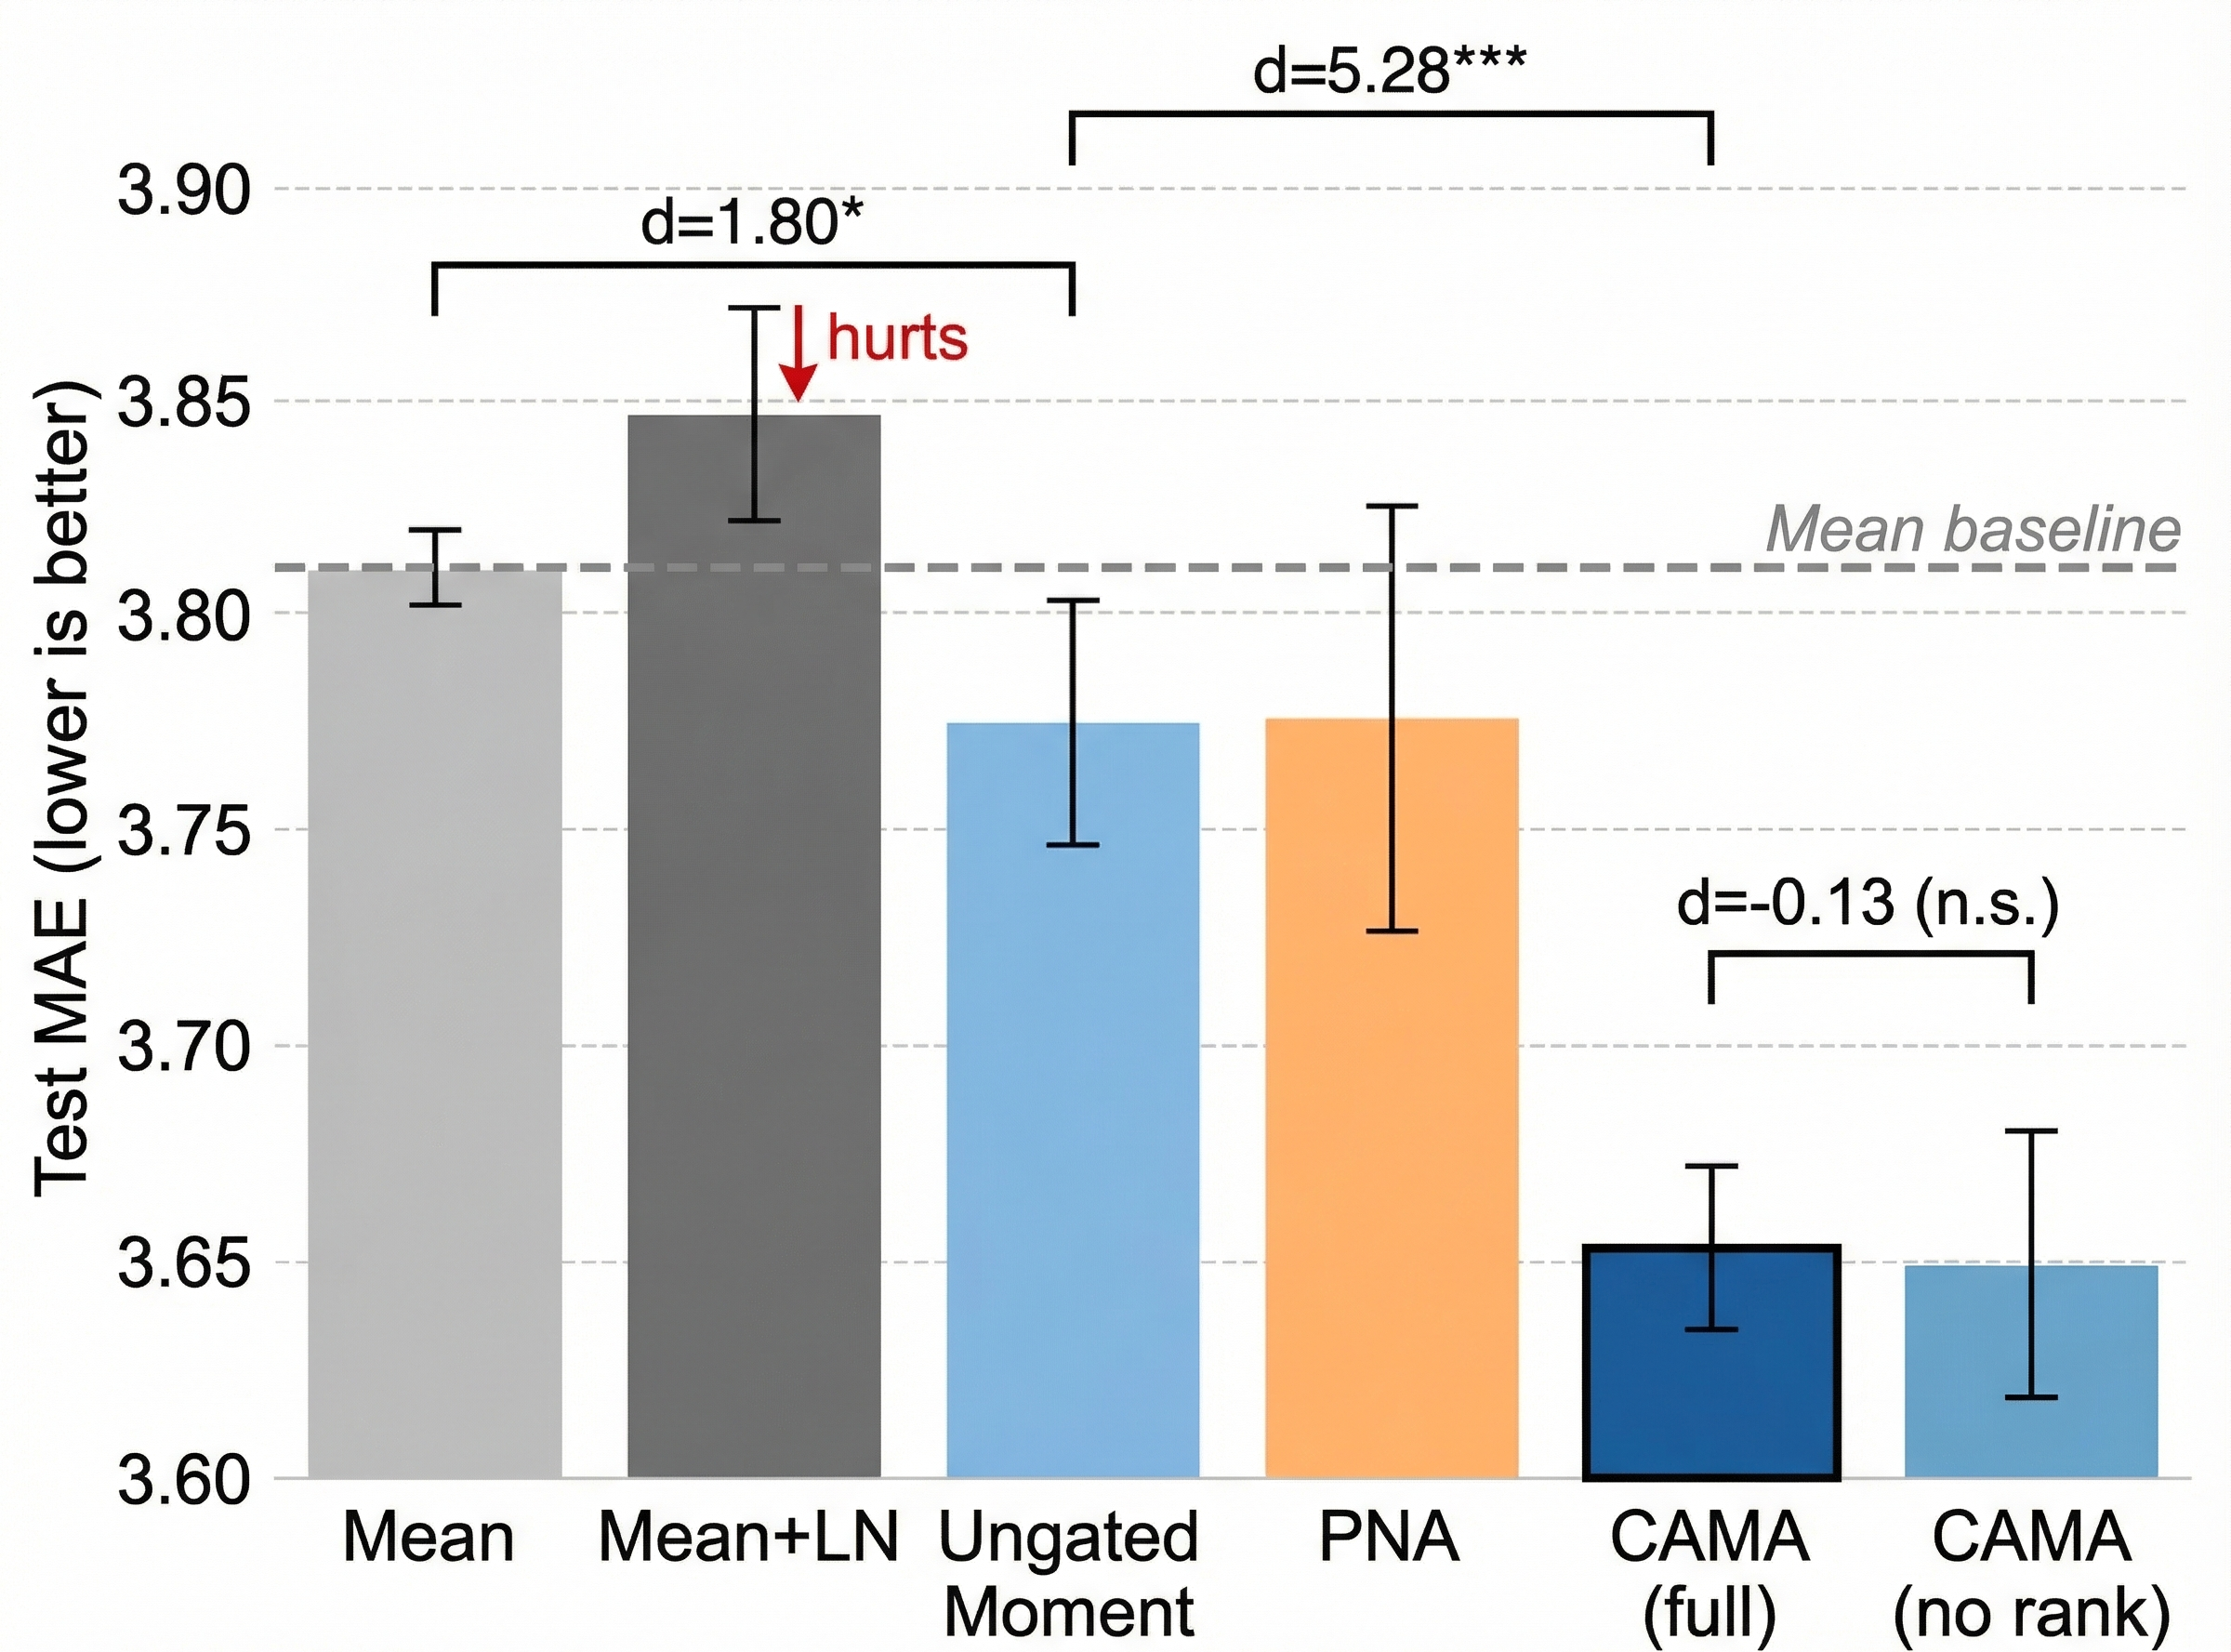
\includegraphics[width=0.92\textwidth,max height=0.4\textheight]{figures/fig_3_v0.png}
  \caption{Component ablation on rel-f1/driver-position (MAE, lower is better). Each bar represents a different aggregation method evaluated over 5 seeds. Error bars show $\pm 1$ standard deviation. Variance injection improves over standard mean ($d = 1.80$, $p = 0.016$). Cardinality-based gating improves further ($d = 5.28$, $p < 10^{-4}$). Spectral rank conditioning adds no value: CAMA (no rank) matches CAMA (full) ($d = -0.13$, $p = 0.83$). CAMA outperforms PNA ($d = 3.25$, $p < 0.001$). LayerNorm degrades performance.}
  \label{fig:ablation}
\end{figure}

Four findings emerge from the ablation. (i)~\textbf{Variance injection helps}: ungated moment injection ($\mu + W_\sigma \sigma^2$) significantly improves over standard mean ($d = 1.80$, $p = 0.016$), confirming that per-dimension variance carries task-relevant information that mean pooling discards. (ii)~\textbf{Gating improves further}: CAMA (full) significantly outperforms ungated injection ($d = 5.28$, $p < 10^{-4}$), demonstrating that cardinality-dependent control of variance injection is better than always-on injection. (iii)~\textbf{Rank conditioning adds nothing}: the no-rank ablation performs identically to CAMA full ($d = -0.13$, $p = 0.83$), confirming that the effective spectral rank signal provides no information beyond cardinality alone. This motivated our pivot from ``Rank-Aware'' (RAMA) to ``Cardinality-Aware'' (CAMA) framing. (iv)~\textbf{CAMA outperforms PNA}: CAMA significantly beats PNA-style multi-aggregation ($d = 3.25$, $p < 0.001$), demonstrating that adaptive gated variance injection is more effective than uniform multi-aggregation for FK joins. Additionally, LayerNorm \emph{hurts} performance ($d = -2.12$, $p = 0.007$), ruling out normalization as a confounding explanation.

\subsection{Sum-Aggregation Comparison}
\label{sec:sum_comparison}

A key question is whether CAMA merely recovers what sum aggregation provides for free. We compare all three methods on the tasks where sum baselines are available.

On rel-stack/user-engagement (classification, 3 seeds): CAMA achieves AP = $0.401 \pm 0.001$, sum achieves AP = $0.400 \pm 0.001$, and mean achieves AP = $0.379 \pm 0.005$. CAMA outperforms sum ($d = 1.63$) and strongly outperforms mean ($d = 5.14$). On rel-amazon/item-ltv (regression, val-only): CAMA achieves MAE = $46.97 \pm 0.05$, sum achieves MAE = $47.33 \pm 0.38$, and mean achieves MAE = $51.80 \pm 0.39$. CAMA edges sum ($d = 1.21$) and strongly outperforms mean ($d = 17.28$). The pooled CAMA-vs-sum effect across 6 comparisons is $d = 0.39$ (95\% CI: $[-0.61, 1.38]$, $p = 0.45$, $I^2 = 64.9\%$) with $P(\text{CAMA} > \text{sum}) = 0.775$. The evidence suggests that CAMA brings mean-aggregation architectures to \emph{parity} with sum rather than \emph{surpassing} sum, which is the intended contribution: recovering distributional information through principled enrichment rather than magnitude-preserving summation.

\subsection{Information Compression Measurement}
\label{sec:compression}

To validate the information compression motivation, we instrument HeteroGraphSAGE during inference to measure effective rank before and after mean aggregation at each FK edge type across three contrasting tasks. The mean compression ratio (ratio of aggregated effective rank to child-set effective rank) is 0.84 across 97 edge-type measurements, confirming that mean aggregation discards approximately 16\% of representational diversity at each FK step. We also validate a cheap $O(Nd)$ variance-entropy proxy against SVD-based effective rank, obtaining a mean Spearman correlation of $\rho = 0.63$ across tasks. The correlation between compression severity and CAMA benefit is $\rho = -0.5$ across 3 tasks (directionally consistent: more compression correlates with greater CAMA benefit, but underpowered with only 3 data points).

Notably, a comparison of effective rank under mean vs.\ sum aggregation yielded a surprising result: mean produces \emph{higher} effective rank than sum (ratio 0.978). The information that sum preserves operates through magnitude scaling rather than rank, and the distributional information that CAMA recovers (per-dimension variance) is distinct from the spectral rank structure. This finding led us to frame CAMA's mechanism as ``distributional information loss'' rather than ``rank collapse.''

\subsection{RelGNN Scope Validation}
\label{sec:relgnn}

To validate our scope claim that CAMA targets mean-aggregation architectures specifically, we integrate CAMA into RelGNN's \citep{Chen2025} SAGEConv aggregation on two regression tasks (Table~\ref{tab:relgnn}).

\begin{table}[!htbp]
\centering
\caption{Scope validation---RelGNN with and without CAMA.}
\label{tab:relgnn}
\small
\begin{tabular}{@{}lllll@{}}
\toprule
Task & RelGNN (MAE $\downarrow$) & RelGNN + CAMA (MAE $\downarrow$) & $d$ & $p$ \\
\midrule
rel-f1 / driver-position & $4.28 \pm 0.27$ & $4.38 \pm 0.27$ & $-0.35$ & 0.56 \\
rel-amazon / item-ltv & $57.57 \pm 1.69$ & $57.99 \pm 0.86$ & $-0.31$ & 0.43 \\
\midrule
\textbf{Pooled} & --- & --- & $\mathbf{-0.33}$ & --- \\
\bottomrule
\end{tabular}
\end{table}

CAMA provides no benefit when integrated into RelGNN (pooled $d = -0.33$, $I^2 = 0\%$), with gate values remaining at their initialization (${\sim}0.50$) throughout training. RelGNN's multi-head attention-weighted aggregation already produces non-uniform, diversity-preserving combinations of child embeddings, rendering CAMA's variance injection redundant. This null result is not a limitation but a \emph{scope confirmation}: CAMA addresses information compression at mean aggregation, which does not occur in attention-based architectures.


%% ============================================================
\section{Discussion and Limitations}
\label{sec:discussion}

\subsection{When Does CAMA Help?}
\label{sec:when}

CAMA's benefits concentrate under two conditions. First, \emph{classification tasks}, where the distributional diversity of an FK group is directly predictive of categorical outcomes. For example, a user whose purchase history spans many product categories (high per-dimension variance) may have different engagement probability than one with homogeneous activity; the variance signal directly encodes this diversity. For regression tasks predicting continuous values, the relationship between distributional spread and the target is weaker, explaining CAMA's null regression effect. Second, \emph{mean-aggregation architectures}, where distributional information is truly discarded. Architectures using sum (which preserves magnitude) or attention (which weights neighbors non-uniformly) already retain aspects of distributional structure, rendering CAMA's enrichment redundant.

\subsection{Relationship to Predictive Residual Message Passing}
\label{sec:prmp}

The prior Predictive Residual Message Passing (PRMP) approach attempted to inject diversity by subtracting predicted embeddings from actual messages before aggregation. PRMP's ablations revealed a paradox: random and frozen predictions performed comparably to learned ones. This paradox resolves naturally under the CAMA framework: \emph{any} subtraction from the mean diversifies the aggregated representation, regardless of prediction quality. What mattered was not the prediction but the injection of distributional information. CAMA directly measures and injects the relevant diversity signal (per-dimension variance), eliminating the prediction MLP and the paradox entirely.

\subsection{Limitations}
\label{sec:limitations}

We report limitations concretely:

\begin{enumerate}
    \item \textbf{Classification-specific benefit.} CAMA shows null regression effects ($d = 0.23$, $p = 0.81$). Only 3 classification tasks were evaluated; additional classification benchmarks are needed to confirm the finding.

    \item \textbf{Gate stasis.} Learned gate values remain near their 0.5 initialization for 81\% of edge types, suggesting the gate gradient signal is weak in most cases. The Amazon dataset is an exception where gates diverge meaningfully at 10 epochs. An experiment comparing fixed gate values to learned gates would determine whether the learning dynamics require improvement.

    \item \textbf{Val-only evaluation.} The rel-amazon/item-ltv results ($d = 13.58$) use validation-set MAE because RelBench withholds test labels. Validation-based evaluation may inflate or deflate effect sizes.

    \item \textbf{Epoch sensitivity.} At 5 training epochs, CAMA shows \emph{negative} effects on Amazon ($d = -1.38$), while at 10 epochs the effect reverses to strongly positive ($d = 13.58$). CAMA's gate requires sufficient training time to learn meaningful behavior.

    \item \textbf{No SOTA integration benefit.} CAMA provides no improvement when integrated into RelGNN \citep{Chen2025} ($d = -0.33$), limiting applicability to mean-aggregation architectures.

    \item \textbf{Sum baseline threat.} The pooled CAMA-vs-sum effect ($d = 0.39$, $p = 0.45$) is not significant. On some tasks, sum aggregation matches CAMA's performance without additional parameters.
\end{enumerate}


%% ============================================================
\section{Conclusion}
\label{sec:conclusion}

Information compression at foreign-key joins is a measurable bottleneck for mean-aggregation GNN architectures in relational deep learning: mean pooling discards per-dimension variance that encodes the diversity profile of each FK group. CAMA addresses this through gated variance injection conditioned on FK-group cardinality, enriching mean aggregation with second-moment information while maintaining a safe default at low cardinality. Across 8 RelBench entity-level tasks on 5 databases, CAMA demonstrates a pooled Cohen's $d$ of 0.88 overall, decomposing into a large classification-specific benefit ($d = 2.13$, 100\% positive sign consistency) and a null regression effect ($d = 0.23$). On classification benchmarks, CAMA brings mean-aggregation architectures to parity with sum-based alternatives ($d = 1.63$ on user-engagement, $d = 1.21$ on item-ltv), providing a principled enrichment that preserves mean's stability while recovering distributional information that mean pooling discards. The controlled ablation confirms that variance injection is the primary mechanism and cardinality-based gating improves further, while spectral rank conditioning is unnecessary.

CAMA is a lightweight, model-agnostic module: one scalar gate and one $d \times d$ projection per edge type, requiring no architectural changes and integrating as a one-line drop-in replacement for mean aggregation in PyTorch Geometric. Future work should extend evaluation to additional classification tasks to strengthen the subgroup analysis, investigate gate learning dynamics to resolve the 81\% stasis phenomenon, and explore CAMA's interaction with deeper GNN architectures where within-step compression and depth-wise rank collapse \citep{Roth2024a} may compound.

\bibliography{references}

\end{document}
